%----------------------------------------------------------------------------------------
%	PACKAGES AND OTHER DOCUMENT CONFIGURATIONS
%----------------------------------------------------------------------------------------

\documentclass[12pt]{article}
\usepackage{alltt}
\usepackage[spanish]{babel}
%\usepackage[extreme]{savetrees}
\usepackage[
   % showframe,
    paper=letterpaper,
    headheight=54.45pt,
    bottom=1.2in
]{geometry}
\usepackage[utf8]{inputenc}
\usepackage{fancyhdr} % Required for custom headers
\usepackage{graphicx}
\usepackage{lastpage} % Required to determine the last page for the footer
\usepackage{setspace}
\usepackage{hyperref}
\usepackage[theoremfont,largesc,tighter,osf]{newpxtext}
\usepackage{xcolor}

%%%%%%%%% === Document Configuration === %%%%%%%%%%%%%%

\pagestyle{fancy}
\lhead{

\includegraphics[width=0.2\textwidth]{../../Logos/FEUCR.pdf}
} % Top left header
\chead{} % Top center header
\rhead{

\includegraphics[clip, trim=1.3cm 16.3cm 11.85cm 0.5cm, width=0.07\textwidth]{../../Logos/SF.pdf}
} % Top right header
\lfoot{} % Bottom left footer
\cfoot{Secretaría de Finanzas, FEUCR.\\
        Ciudad Universitaria Rodrigo Facio,
        costado oeste del comedor estudiantil.\\
        {\bfseries Teléfono:} (506) 2511-4615\quad
        {\bfseries E-mail:} \texttt{finanzas.feucr@ucr.ac.cr}
       } % Bottom center footer
\rfoot{P\'ag.\ \thepage\ de\ \pageref{LastPage}
       } % Bottom right footer

\renewcommand{\footrulewidth}{0.3pt}% default is 0pt
\renewcommand{\headrulewidth}{0.3pt}% default is 0pt
\def\baselinestretch{1.5}% Interlineado
\setlength{\parindent}{0.09\linewidth}% Sangria

\newskip\smallskipamount \smallskipamount=6pt plus 2pt minus 2pt
\newskip\medskipamount   \medskipamount  =12pt plus 4pt minus 4pt
\newskip\bigskipamount   \bigskipamount =18pt plus 6pt minus 6pt

\newcommand{\MONTH}{%
  \ifcase\the\month
  \or enero% 1
  \or febrero% 2
  \or marzo% 3
  \or abril% 4
  \or mayo% 5
  \or junio% 6
  \or julio% 7
  \or agosto% 8
  \or septiembre% 9
  \or octubre% 10
  \or noviembre% 11
  \or diciembre% 12
  \fi}

\newenvironment{significant}{\begin{center}\begin{minipage}{0.9\textwidth}\centering\em}{\end{minipage}\end{center}}

%----------------------------------------------------------------------------------------
%	ARTICLE CONTENTS
%----------------------------------------------------------------------------------------
\begin{document}


\begin{flushright}
  %\textcolor{white}{\textbf{CONSECUTIVO}}\\
  Circular-SF-2-2021\\
  \medskip
  \the\day\ de \MONTH, \the\year
\end{flushright}
\medskip
\begin{flushleft}\begin{spacing}{1}
  \textbf{Tesorerías\\
  Órganos Federativos\\
  Asociaciones Federadas\\
  Federación de Estudiantes de la Universidad de Costa Rica}
\end{spacing}\end{flushleft}

\noindent Estimados tesoreros:\par

Cordial saludo de mi parte.\par
Respecto al proceso de solicitudes de órdenes de servicio tomen debida nota que los pagos de la Federación de Estudiantes se tramitan a través del sistema GECO de la Oficina de
Suministros (OSUM) de la Universidad de Costa Rica. Por este motivo, toda persona física o jurídica que
desee ofrecer servicios, debe registrarse previamente y por una única vez, de la siguiente forma: 

\begin{significant}
Se debe hacer el registro con la mayor antelación posible para evacuar las dudas que haya con tiempo, y
se debe hacer \underline{previo a haber emitido la factura} o prestado el servicio para registrarse.
\end{significant}


\section{Registro de proveedores en GECO}

\begin{enumerate}
    \item Acceder a la página web \textcolor{blue}{\href{https://geco.ucr.ac.cr/geco/}{https://geco.ucr.ac.cr/geco/}}
    \item Registrarse en la pestaña de "Proveedores". 
    \begin{center}
        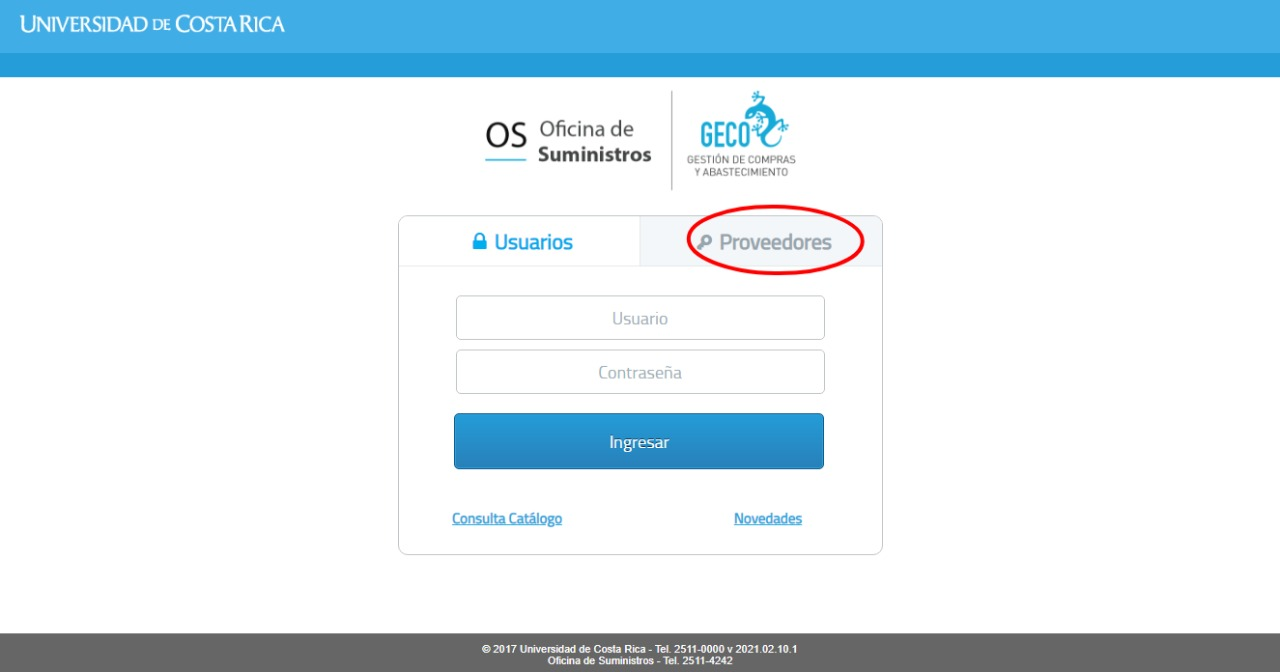
\includegraphics[width=0.55\textwidth]{Oficios/Circular-SF-2-2021/geco1.jpg}
    \end{center}
    \item Registrar la información de quien emite la factura (los datos de cuenta deben pertenecerle).
    \item Las pestañas obligatorias son: 
    \begin{enumerate}
        \item Información personal.
        \begin{center}
        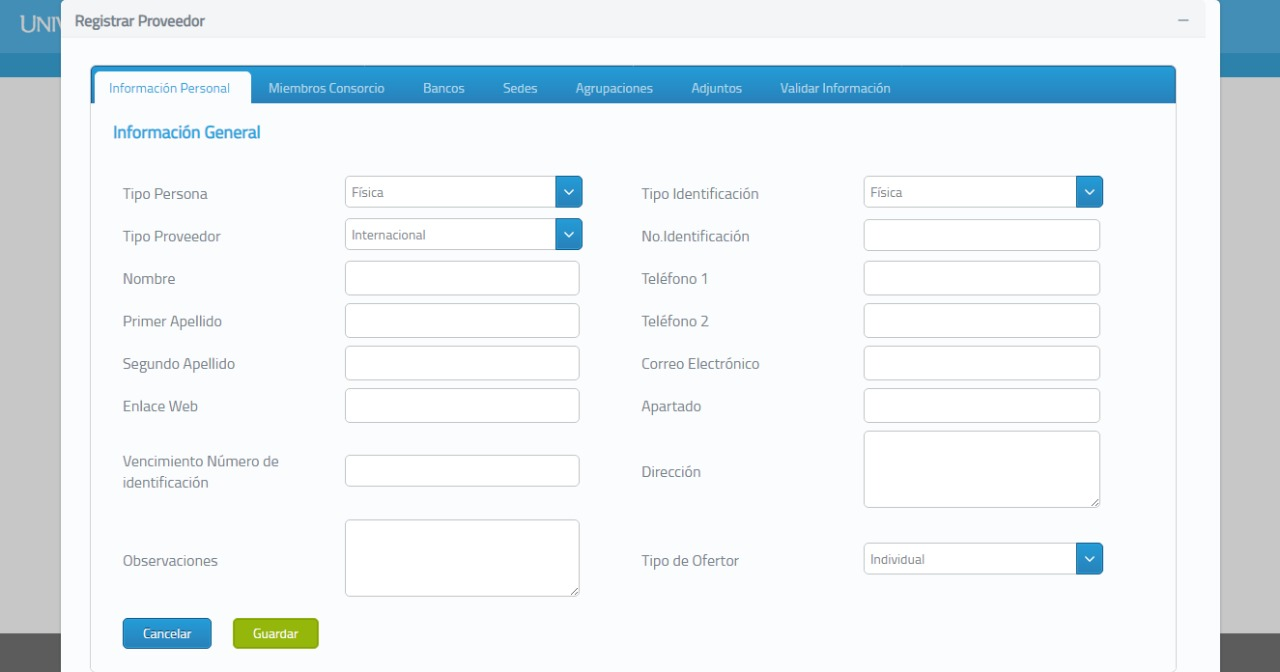
\includegraphics[width=0.6942\textwidth]{Oficios/Circular-SF-2-2021/geco2.jpg}
    \end{center}
        \item Bancos (código Swift no se debe indicar). La cuenta debe ser en \textbf{colones únicamente}.
        \begin{center}
        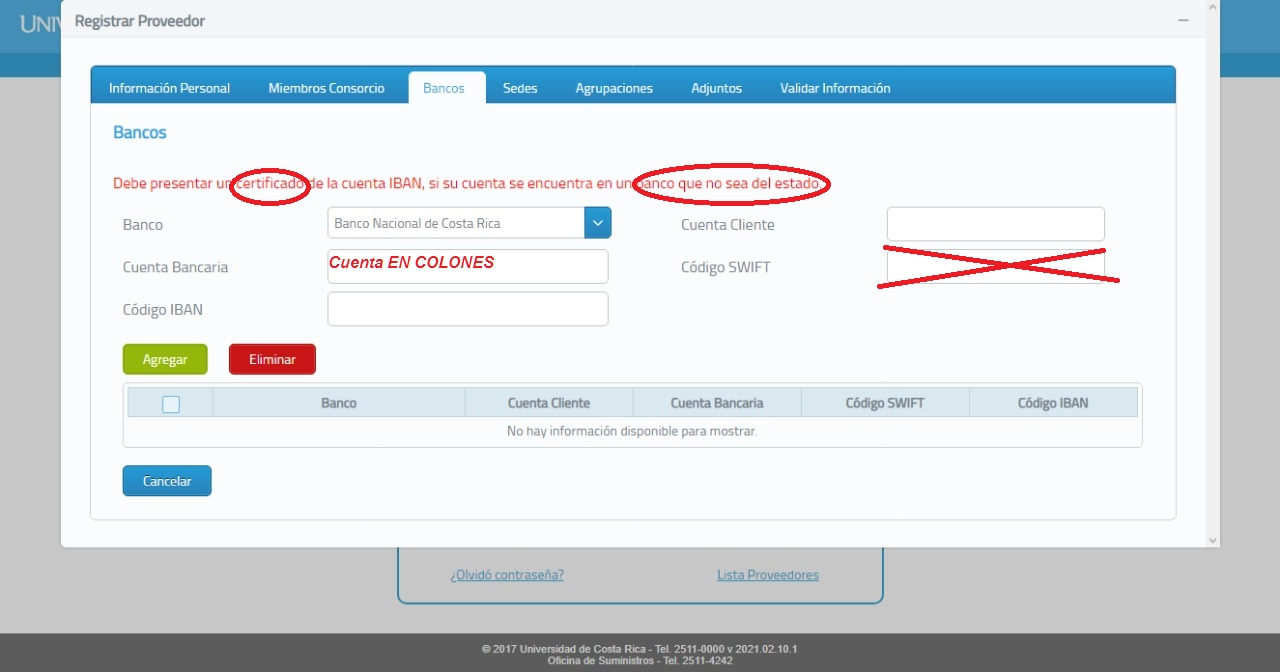
\includegraphics[width=0.6942\textwidth]{Oficios/Circular-SF-2-2021/geco3.jpg}
    \end{center}
        \newpage 
        \item Sedes (indicar “Rodrigo Facio”).
        \begin{center}
        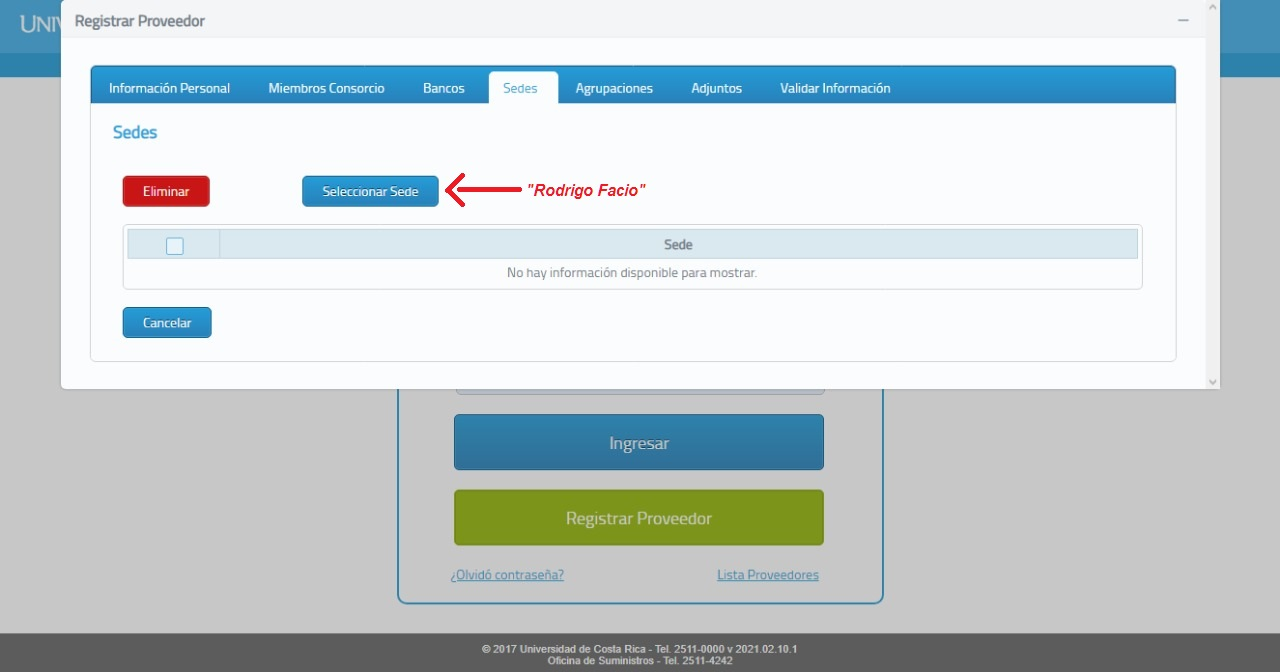
\includegraphics[width=0.6942\textwidth]{Oficios/Circular-SF-2-2021/geco4.jpg}
    \end{center}
        \item En la pestaña ``Adjuntos'', agregar copia de cédula y certificado de cuenta IBAN en caso de Bancos Privados.
        \begin{center}
        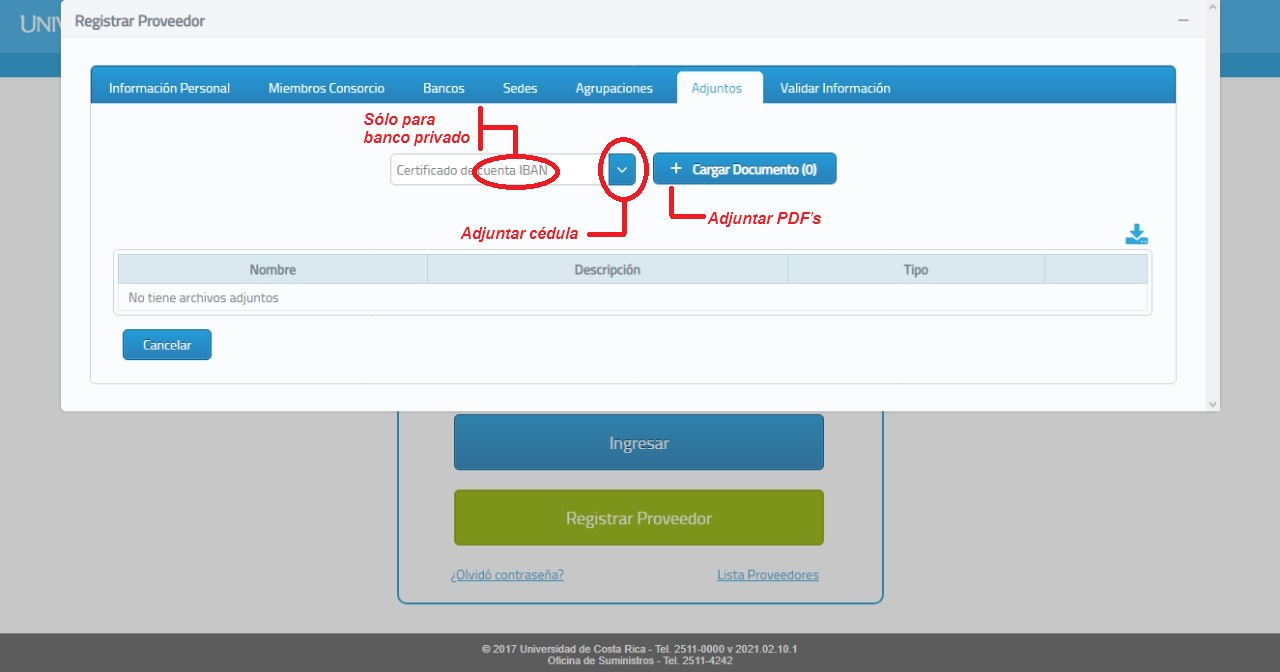
\includegraphics[width=0.6942\textwidth]{Oficios/Circular-SF-2-2021/geco5.jpg}
    \end{center}
    \end{enumerate}
    \item Una vez realizado el registro, recibirá un correo electrónico de parte de la dirección \textcolor{blue}{\href{mailto:geco@ucr.ac.cr}{geco@ucr.ac.cr}}. Una vez recibida esta confirmación, favor notificar al correo del tesorero correspondiente de la Asociación u Órgano, especificando el nombre completo del proveedor registrado (cuyo
nombre es el mismo del emisor de la factura) y así proceder con el trámite
correspondiente.
    \item En caso de dudas escribir a la dirección \textcolor{blue}{\href{mailto:giovanni.masis@ucr.ac.cr}{giovanni.masis@ucr.ac.cr}}
    o llamar al señor Giovanni Masís al teléfono 2511-2951.
    \item La declaración jurada que se solicita deberá serle entregada por la persona que le contrata el servicio y debe indicarle si la persona que emite la factura tiene cédula \underline{física o jurídica}.

\end{enumerate}

Una vez completado el registro en GECO, se debe entregar la factura con los siguientes requisitos:

\section{Emisión de proforma previo a la facturación}

Una vez que la Asociación u Órgano formalice la contratación del servicio, el proveedor del servicio deberá enviarle una factura-proforma al tesorero correspondiente con la descripción del servicio contratado, el monto subtotal (sin IVA) y total (con IVA).\par 
El envío de la proforma es \textbf{obligatorio} y si no se cuenta con una, no se puede tramitar la orden de servicio. La proforma se debe enviar \textbf{antes que la factura}. Detallo puntualmente los datos pedidos en la proforma a continuación:

\begin{enumerate}
    \item Nombre de la sociedad o del proveedor.
    \item Número de cédula de identidad, o cédula jurídica, según corresponda.
    \item Número de \textbf{cuenta IBAN}, junto con el nombre del banco al que corresponde.
    \item Una \textbf{descripción detallada} del servicio o desglose de gastos finales.
    \item Debe ser emitada a nombre de: \textbf{Universidad de Costa Rica}, cédula jurídica: \textbf{4-0000-42149}.
    \item El monto subtotal (sin IVA) y total (con IVA) que no debe sufrir alteraciones futuras.
\end{enumerate}

Es de \emph{suma importancia} que el monto detallado dentro de la proforma \textbf{no sufra alteraciones} a la hora de entregar la factura. Caso que sí, el proceso debe reiniciarse, la factura se debe cancelar y se debe enviar una nueva proforma con el monto corregido. 

\section{Facturación}

Las facturas deben emitirse una vez que el sistema de la Universidad les envíe mediante correo
electrónico la Orden de Compra de Servicios (OCS), cualquier factura emitida previamente a esto, \textbf{tendrá que anularse}.\par  

Las facturas deberán cumplir con los siguientes requisitos:

\subsection{Régimen Simplificado de Tributación}

\begin{significant}
Existe la posibilidad de hacer uso de facturación electrónica. Si la factura es física deberá incluir una leyenda impresa (no se aceptan sellos) que haga explícito que el proveedor se encuentra acogido al régimen de tributación simplificado.
\end{significant}

Las facturas del \textbf{régimen simplificado} deben cumplir con los siguientes requisitos: 

\begin{enumerate}
    \item El nombre del cliente será únicamente “\textbf{Universidad de Costa Rica}”, cédula jurídica
\textbf{4-0000-42149}.
    \item Debe incluir una \textbf{descripción clara y detallada} del servicio.
    \item Si factura electrónicamente, debe cumplir con las indicaciones del apartado de régimen
simplificado, \underline{a excepción del 2$\%$ del IVA}, pero deberá adjuntar con el PDF de la factura junto con una
captura de pantalla de la página del Ministerio de Hacienda en donde conste que el proveedor no paga el
IVA.
    \item Fecha de emisión debe ser del día de la prestación del servicio o posterior.
    \item La factura no debe tener tachones.
    \item El emisor de la factura \textbf{debe ser el mismo} que el propietario de la cuenta registrada en GECO.
    \item Cuenta bancaria \textbf{en colones únicamente}.
    \item Si es la primera vez que se tramita el pago desde la sede Rodrigo Facio y mediante Orden de Servicio, debe indicar en la casilla de observaciones de la factura el número IBAN de la cuenta, ya que el pago se realiza mediante transferencia bancaria, \textbf{únicamente}.
\end{enumerate}

Agrego nuevamente que si el monto en la factura no coincide con el monto en la proforma, debe anularse la factura y \textbf{se debe reiniciar el proceso} con una proforma con el monto correcto.

\subsection{Régimen Tradicional de Tributación}

Las facturas del \textbf{régimen tradicional} deben cumplir con los siguientes requisitos: 

\begin{enumerate}
    \item La factura será electrónica \textbf{únicamente}. No se aceptan notas de crédito ni débito.
    \item El nombre del cliente será únicamente “\textbf{Universidad de Costa Rica}”, cédula jurídica
\textbf{4-0000-42149}.
    \item Debe incluir una \textbf{descripción clara y detallada} del servicio.
    \item La clave de factura y el número consecutivo electrónico deben ser claramente visibles.
    \item Fecha de emisión debe ser del día de la prestación del servicio o posterior.
    \item El emisor de la factura \textbf{debe ser el mismo} que el propietario de la cuenta registrada en GECO.
    \item Debió registrar una cuenta bancaria \textbf{en colones únicamente}.
    \item Debe indicar lo siguiente en las “Observaciones” u otro lugar de la factura:
\emph{Federación de Estudiantes de la Universidad de Costa Rica. Fondo de Trabajo 416}.
    \item La factura debe incluir el 2\% de IVA, el monto de este impuesto no debe ser menor ni mayor a ese.
\end{enumerate}

La recepción de facturas electrónicas (junto con los documentos adicionales que se generan) será únicamente al correo de la OAF: \textcolor{blue}{\href{mailto:facturaelectronica.oaf@ucr.ac.cr}{facturaelectronica.oaf@ucr.ac.cr}} (indicarle al proveedor
que, simultáneamente, \underline{descargue el pdf} y \underline{lo adjunte} al correo del \underline{tesorero correspondiente} de la Asociación u Órgano).\par

Agrego nuevamente que si el monto en la factura no coincide con el monto en la proforma, debe anularse la factura y \textbf{se debe reiniciar el proceso} con una proforma con el monto correcto.

\section{Notas Adicionales}

\begin{itemize}
    \item Las transferencias tardan entre 20-30 días naturales a partir del día en el que llegan a la
    Vicerrectoría de Vida Estudiantil, no a partir de que se entregan a los órganos respectivos dela FEUCR.
    \item Cualquier omisión en el cumplimiento de los requisitos arriba especificados, puede traducirse
en retrasos en la fecha del pago.
    \item Las tesorerías de la unidad contratante deben acompañar, en el endose como texto en el correo, una descripción de la actividad, número y tipo de población asistente para las facturas por servicios de alimentación. A su vez, dichas facturas se deben entregar de manera electrónica dentro la \textbf{plataforma de la Contraloría Estudiantil}.
    \item En caso de atrasos en el proceso de entrega de la factura a la Contraloría, deben apegarse a las indicaciones que el órgano brinde. 
    \item Se notificará al proveedor sobre errores o correcciones que deban hacerse para terminar el trámite de pago, las cuales deberán ser resueltas en un plazo máximo de 30 días naturales, posteriores a los cuales la institución dará por caducado el proceso de pago.
\end{itemize}

Sin más les deseo muchos éxitos con la venida de este nuevo periodo, se despide cordialmente,\par
\bigskip
\bigskip
\bigskip
\begin{spacing}{1}
\textit{\textbf{Jonathan Josué Carcache Ríos}}\par
\textit{Coordinación}\\
\textit{Secretaria de Finanzas}
\end{spacing}
\medskip
\begin{flushleft}\begin{spacing}{1}
 \scriptsize{CC. Archivo/JIRR

 }
\end{spacing}\end{flushleft}
%%%%%%%%%%%% Contents end %%%%%%%%%%%%%%%%
%Indent whole paragrah: https://tex.stackexchange.com/questions/35933/indenting-a-whole-paragraph
%Dates: https://tex.stackexchange.com/questions/185548/the-year-in-roman-and-the-month-in-text
%SKIPS:https://tex.stackexchange.com/questions/41476/lengths-and-when-to-use-them/41488
%SKIPS2: https://tex.stackexchange.com/questions/476/what-if-anything-is-the-advantage-of-bigskip-and-friends-over-vspace
%%%%%%%%%%%%%%%%%%%%%%%%%%%%%%%%%%%%%%%%%%
%\newpage
%\nocite{*}
%\bibliographystyle{plain}
%\bibliography{bibi}
\end{document} 